 \section{Durchführung der Extraktion und Konstruktion der Features} \label{secc:Umsetz Featextr}
Die Umsetzung der Feature-Extraktion erfolgt mit dem Wissen, dass sie zwei Funktionen Erfüllen muss. Zum Einen werden Features benötigt, als Prozessschritt im Machine Learning Workflow und zum Anderen benötigt das fertige Modul eine Vorverarbeitung. Die Durchführung der Extraktion wird deshalb direkt so Implementiert, dass sie sich einfach in das Modul zur Verhaltensklassifikation integrieren lässt. Nach der Feature-Auswahl sollen lediglich kleine Anpassungen notwendig sein, um die Extraktion in das Modul einfügen zu können. Ergebnis dieses Kapitels ist die Struktur für die komplette Vorverarbeitung des Moduls (\autoref{sec:Meth FinalKonzept}).\par

Im ersten Schritt sind jedoch die Features zu den Ereignisintervallen (\autoref{sec:Meth Datensatz}) zu extrahieren, um mit diesen in die Feature-Konstruktion zu gehen und anschließend in die Feature-Auswahl. Nach der Verifizierung werden die Ereignisse in Intervalle zerteilt, wie in \autoref{sec:Meth Datensatz} beschrieben. Aus diesem Grund wird sich in der Feature-Extraktion immer auf die Ereignisintervalle bezogen. Extrahiert werden zunächst die Basis-Features (\autoref{sec:Meth KonstrFeatures}). In der Konstruktion werden die restlichen Feature-Kategorien generiert. Nach der Feature-Auswahl muss die Extraktion so angepasst werden, dass nicht nur die Basis-Features berechnet werden. Die notwendigen Konstruktionen der Features aus anderen Kategorien sind der Extraktion hinzuzufügen. \par

Der erste Abschnitt erläutert den Prozess, wie die Intervalle gehandhabt werden, um aus diesen die Features zu extrahieren. Im zweiten Abschnitt wird der modulare Aufbau der Feature-Extraktion dargestellt. Der dritte Abschnitt befasst sich mit der konkreten Berechnung der Features. Auch das Assoziationsmodul wird hier beschrieben. Abschließen tut das Kapitel mit der Feature-Konstruktion. 



\subsection{Feature-Extraktion der Ereignisintervalle} \label{sec:Umse ExtrIntervalls}

\begin{figure}[p]
    \centering
    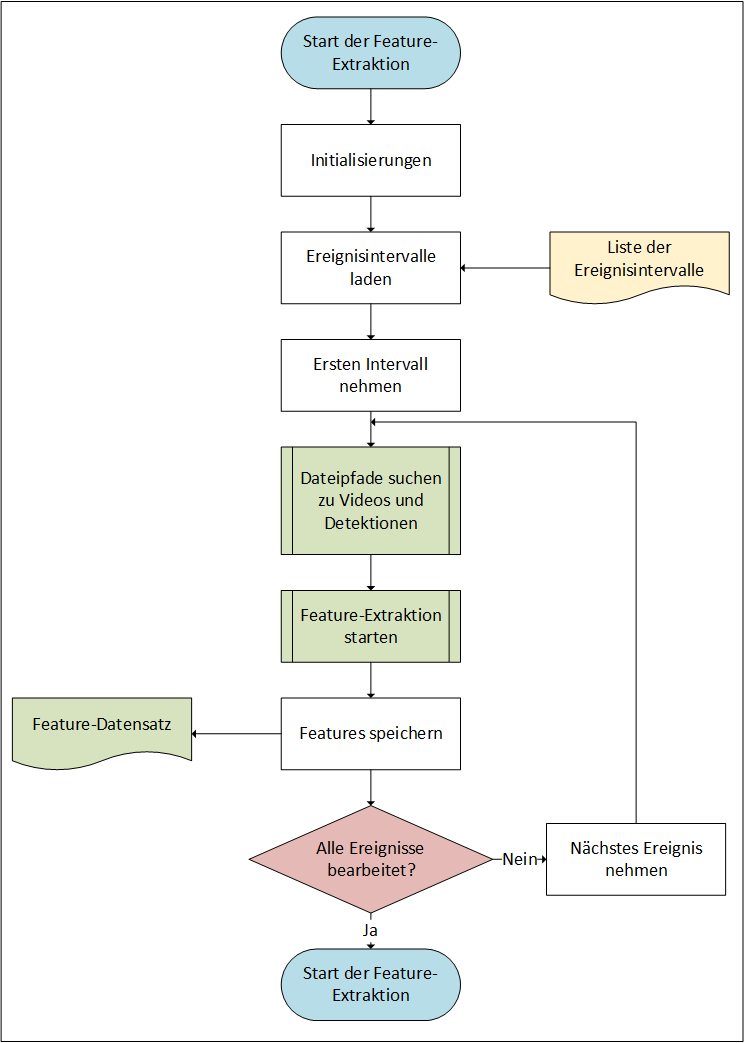
\includegraphics[height=0.9\textheight]{img/Grafiken/Flussdiagramm Feature-Extraktion Start.png}
    \caption{Flussdiagramm der Steuerung der Feature-Extraktion der Ereignisintervalle.}
    \label{fig:FlussDia Intervalle}
\end{figure}

Die Ereignisintervalle sind in einer csv-Datei gespeichert. Jede Zeile der Datei beinhaltet die Informationen zu einem Intervall. Das sind der Start- und der Endzeitpunkt, die Kamera ID und das Label der Verhaltensweise. Zu jedem Intervall muss eine Feature-Extraktion durchgeführt werden. Das Flussdiagramm in \autoref{fig:FlussDia Intervalle} zeigt, den Ablauf dieses Prozesses. \par

Zum Laden der Ereignisintervalle wird die \textit{Pandas} Bibliothek verwendet. Um die Features zu Extrahieren werden die Detektionsdaten, sowie das Video benötigt. Diese Dateien werden wieder mit dem Modul \textit{FileSearch} herausgesucht, welches auch in \autoref{sec:Umsetz VeriInterfaceEbene} angewendet wird. Der codeauszug \ref{lst:FE BibsNloadInter} zeigt das Laden der Bibliotheken und das Laden der Ereignisintervalle.\par

\begin{pythoncode}{Bibliotheken Importieren und Ereignisintervalle laden}{lst:FE BibsNloadInter}
#Bibliotheken Laden
from FileSearch import FileSearch
import pandas as pd

#Laden der Ereignisintervalle
ereignisIntervalle = pd.read_csv("ereignisse_intervalle.csv")
\end{pythoncode}

Anschließend wird ein Objekt der \textit{FeatureExtractor}-Klasse initialisiert. Die \textit{FeatureExtractor}-Klasse ist ein Modul, welches die Vorverarbeitung, sowie die Feature-Extraktion implementiert hat. Es kann hier modular in den Prozess integriert werden. Der Codeauszug \ref{lst:FE InitFeatExtr} zeigt die Initialisierung eines \textit{FeatureExtractors}. Auf die Implementation der \textit{FeatureExtractor}-Klasse wird in \autoref{sec:Umsets FeatExtrKlass} eingegangen.

\begin{pythoncode}{Integration und Intitalisierung eines \textit{FeatureExtractors}}{lst:FE InitFeatExtr}
#Initalisieren der Feature-Extraktion
from FeatureExtractor import FeatureExtractor
feat_extr = FeatureExtractor()
\end{pythoncode}

Es wird durch jeden Intervall iteriert. Zu den Intervallen werden die Informationen entgegen genommen und die Dateien werden mittels des \textit{FileSearch} Moduls gesucht. Die Intervallinformationen, sowie die Dateipfade werden der Feature-Extraktion übergeben. Die Feature-Extraktion wird über die Methode \textit{get\_features} des \textit{FeatureExtractors} gestartet. Diese ermittelt die Features zum Intervall und gibt diese zurück. Die Features werden anschließend in einer csv-Datei gespeichert, um sie später für die Konstruktion zu verwenden. Das ist im Codeauszug \ref{lst:FE IterInterv} zu sehen.Das Programm demonstriert die einfache Integration der Vorverarbeitung und der Feature-Extraktion. 

\begin{pythoncode}{Iteration durch die Ereignisintervalle und die Suche der Dateien.}{lst:FE IterInterv}
#Iteration durch jeden Ereignisintervall
for idx, row in ereignisIntervalle.iterrows():

    #Intervall-Infos entgegennehmen
    startTime = str(row['Startzeit'])
    endTime = str(row['Endzeit'])
    kameraID = str(row['KameraID'])
    ereignisLabel = str(row['Label'])

    #Dateien auf Festplatten suchen und Pfade zurückgeben 
    files = FileSearch(startTime, endTime, kameraID)

    #Feature-Extraktion starten
    #Extrahierte Features entgegennehmen
    feat_dict = feat_extr.get_features(files.detectionDataPath, 
                                       files.videofilepath, 
                                       startTime, 
                                       endTime, 
                                       kameraID)

    #Label hinzufügen: Wird für den Labelvektor benötigt
    feat_dict['Label'] = ereignisLabel
    
    #Features in eine csv-Datei schreiben
    append_features_to_dataset(feat_dict)
\end{pythoncode}



\subsection{Implementierung der Feature-Extraktion} \label{sec:Umsets FeatExtrKlass}

\begin{figure}[p]
    \centering
    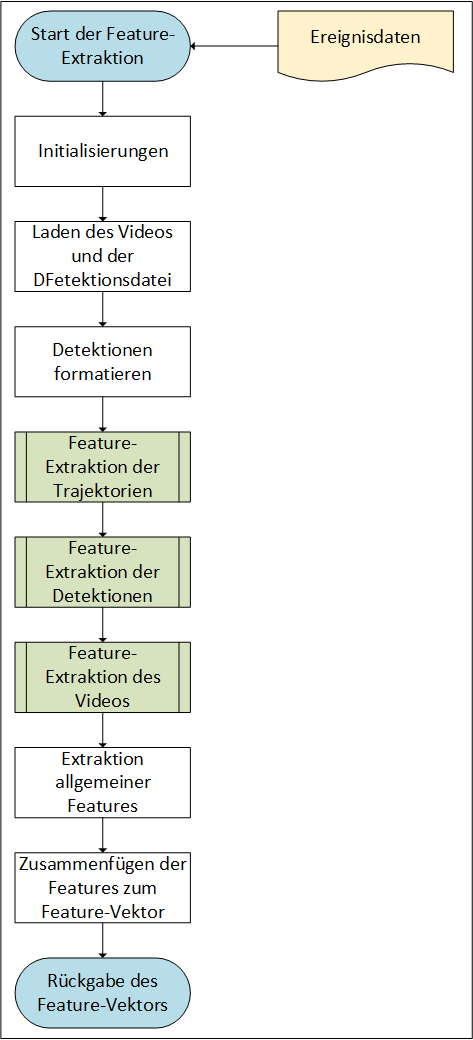
\includegraphics[height=0.9\textheight]{img/Grafiken/Flussdiagramm Feature-Extraktion sammeln.png}
    \caption{Flussdiagramm des Programmablaufs der Feature-Extraktion.}
    \label{fig:FlussDia FeatExtraktion}
\end{figure}

Die Feature-Extraktion ist in einer Python-Klasse implementiert. Die Strukturierung in einer Klasse wird gewählt, um Daten effizient und einfach zugänglich zu machen für die Methoden in der Klasse. Ebenfalls ist die modulare Integration der Extraktion mit einer Klasse übersichtlich zu erreichen. Der Codeauzug \ref{lst:FE ExtrKlassKonst} zeigt den Konstruktor der Klasse. Dieser initialisiert einige Klassen-Variablen. Die Variablen werden während der Extraktion von Klassen-Methoden befüllt. 

\begin{pythoncode}{Konstruktor der \textit{FeatureExtractor}-Klasse.}{lst:FE ExtrKlassKonst}
#Konstruktor der FeatureExtractor-Klasse
class FeatureExtractor:
    def __init__(self):
        self.detektionen = None
        self.startframe = None
        self.endframe = None
\end{pythoncode}

Kern der Feature-Extraktion ist die Methode \textit{get\_features}. Es ist die Methode, welche in \autoref{sec:Umse ExtrIntervalls} die Extraktion zu den Intervallen startet. Sie benötigt die Informationen zu einem Ereignis entgegen, sowie die Pfade zu den benötigten Dateien. Die Detektionen werden Formatiert, wie es in \autoref{sec:Meth FeatExtr} beschrieben ist. Der Code für die Formatierung ist bereits vor dieser Arbeit implementiert worden, weshalb nicht näher drauf eingegangen wird. Das Video wird geladen. Das geschieht mit der \textit{OpenCV} Bibliothek, wie in \autoref{sec:Umsetz VeriEbene}. Der Codeauszug \ref{lst:FE StartExtrakt} zeigt den Start der Methode und das Laden der Dateien. Das Flussdiagramm in der Abbildung \ref{fig:FlussDia FeatExtraktion} zeigt den Ablauf der \textit{get\_features} Methode.

\begin{pythoncode}{Methode zum Starten der Feature-Extraktion.}{lst:FE StartExtrakt}
#Methode zum starten der Extraktion
def get_features(self, detsPath, vidPath, startTime, endTime, kameraID):

    #Laden und Formatieren der Detektionsdaten
    self.detektionen = self.loadDetections(detsPath, startTime, endTime)

    #Laden des Videos mit OpenCV
    import cv2
    self.vidCap = cv2.VideoCapture(vidPath)

\end{pythoncode}

Wie in \autoref{sec:Meth FeatExtr} dargestellt, lässt sich die Feature-Extraktion in Form von drei Submodulen betrachten. Jedes Submodul ist dafür zuständig die Features aus einer bestimmten Datenart zu extrahieren. In der Umsetzung ist dies genau so Implementiert. Es gibt ein spezifisches Extraktormodul für die Trajektorien, für die Detektionen und für das Video. \par 

Im Codeausschnitt \ref{lst:FE SpeziExtra} ist zusehen, dass die Submodule integriert werden. Implementiert sind sie Ebenfalls als Klassen. Sie werden in \autoref{sec:Umsetz SubExtrak} genauer beschrieben. Jedes wird mit den benötigten Informationen initialisiert. Die Methode \textit{extract\_all\_features} startet für alle Submodule die Extraktion.

\begin{pythoncode}{Datenspezifische Extraktoren starten.}{lst:FE SpeziExtra}
#Vorheriger Code innerhalb der get_features Methode...

#Integrieren der Datenspezifischen Extraktoren
from extract_tracks import track_extractor
from extract_detections import detection_extractor
from extract_video import video_extractor

#Extrahieren der Features aus den Trajektorien
feat_trk = track_extractor(self.detections, 
                          startTime, 
                          endTime, 
                          kameraID).extract_all_features()

#Extrahieren der Features aus dem Video
feat_vid = video_extractor(vidCap, 
                           self.startframe, 
                           self.endframe, 
                           kameraID).extract_all_features()

#Extrahieren der Features aus den Detektionen
feat_dets = detection_extractor(self.detections, 
                                startTime, 
                                endTime, 
                                kameraID).extract_all_features()

\end{pythoncode}

Nach der Extraktion werden aus jedem Submodul die Features entgegengenommen. Das Feature \textit{uhrzeit} ist keinem der Submodule zuzuordnen. Es wird deshalb als allgemeines Feature bezeichnet und nach den Submodulen ermittelt. Die \textit{uhrzeit} bezeiht sich auf den Startzeitpunkt eines Intervalls. Sie wird in Unixzeit angegeben. Für jeden Intervall wird der Zeitpunkt auf den 01.01.1970 bezogen. Darüber ist die Uhrzeit tagesunabhängig und die Zeiten sind zwischen den Intervallen vergleichbar. \par

Neben der \textit{uhrzeit}, werden den Features die Informationen zum Intervall beigefügt, um diese Später zuordnen zu können. Das ist für die Auswertung der Simulation (\autoref{sec:Meth Sim}) wichtig und auch für die Erstellung des Feature-Datensatzes. Einige Features sind zu Normalisieren. Das erfolgt nach dem alle Features und Informationen zusammengeführt werden. Anschließend werden die Features zurückgegeben. Der Codeausschnitt \ref{lst:FE KombineNRet} zeigt dies.

\begin{pythoncode}{Features zusammenführen und zurückgeben.}{lst:FE KombineNRet}
#Vorheriger Code innerhalb der get_features Methode...

#Allgemeine Features und Infos für die Zuordnung
uhrzeit = self.convert_to_epoche_unix_timestamp(startTime)
features = dict(Startzeit=startTime, 
                Endzeit=endTime, 
                KameraID=kameraID, 
                uhrzeit=uhrzeit)

#Features zusammenfügen
features.update(feat_trk)
features.update(feat_vid)
features.update(feat_dets)

#Normalisieren der Schrittanzahl-Features 
features = self.get_nomalized_features(features)

#Features zurückgeben
return features
\end{pythoncode}

Nach der Feature-Auswahl sind für das Modul Features aus den Basis-Features zu konstruieren. Das erfolgt ebenfalls noch vor der Rückgabe. Da für die Feature-Extraktion aus den Intervallen erstmals nur die Basis-Features relevant sind, ist dies lediglich ein Hinweis, um die Integration der Feature-Extraktion in das Modul nachvollzeihen zu können. \par

Der Codeausschnitt \ref{lst:FE konstrRet} zeigt, dass zwei Methoden verwendet werden, um die benötigten Features aus der Auswahl zu konstruieren. 

\begin{pythoncode}{Features vor der Rückgabe konstruieren.}{lst:FE konstrRet}
#Vorheriger Code innerhalb der get_features Methode...

#Nach der Feature-Auswahl zusätzlich zum Normalisieren
features = self.get_interactions(features)
features = self.get_binning_features(features)

#Features zurückgeben
return features
\end{pythoncode}



\subsection{Implementierung der Berechnung der Features} \label{sec:Umsetz SubExtrak}

Die Klassen, welche die datenspezifische Extraktion der Features Realisieren sind im Kern gleich aufgebaut. Der Konstruktor nimmt die Daten entgegen, welche für die Extraktion benötigt werden. Und der Aufruf der Methode \textit{extract\_all\_features} startet die Berechnung. Da in den Konstruktoren lediglich Variablen zugewiesen werden, wird sich hier auf die \textit{extract\_all\_features} Methode fokussiert. Zunächst werden die Extraktor-Klassen des Videos und der Detektionsdaten betrachtet. \dubpar

\textbf{Feature-Extraktion des Videos}\par

Der Codeauszug \ref{lst:FE ExtrVid}, zeigt die Methode zu der Feature-Extraktion aus dem Video. Der Verlauf der Pixelveränderung wird in der Methode \textit{get\_pixeländerungen} berechnet. Aus diesem werden die Features berechnet. Dies wird mit Hilfe der Bibliothek \textit{numpy} umgesetzt. \textit{numpy} implementiert eine Vielzahl von Methoden für numerische Rechnungen. Der Codeauszug \ref{lst:FE ExtrVid} zeigt die Implementierung.

\begin{pythoncode}{Methode \textit{extract\_all\_features} der Feature-Extraktion aus dem Video.}{lst:FE ExtrVid}
def extract_all_features(self):

    import numpy as np
        
    #Verlauf der Pixeländerung berechnen 
    pixChanges = self.get_pixeländerungen()

    #Berechnen der Features aus der Pixelveränderung
    features = dict(meanPixAenderung = np.nanmean(pixChanges),
                    stdPixAenderung = np.nanstd(pixChanges),
                    maxPixAenderung = np.max(pixChanges),
                    minPixAenderung = np.min(pixChanges),)
    
    return features

\end{pythoncode}

\dubpar
\textbf{Feature-Extraktion der Detektionen}\par

Die Extraktion aus den Detektionsdaten erfolgt ganz ähnlich. Zum einen wird der Verlauf der Objektanzahl erhoben und über die Methode \textit{get\_free\_area} wird der Verlauf der freien Fläche ermittelt. Anschließend werden über \textit{numpy} die Features berechnet und zurückgegeben. Das zeigt der Codeauschnit \ref{lst:FE ExtrDets}

\begin{pythoncode}{Methode \textit{extract\_all\_features} der Feature-Extraktion aus den Detektionsdaten}{lst:FE ExtrDets}
def extract_all_features(self):

    #Objektanzahl Infos zum Ereignisintervall
    objCnt = self.detections['objectCount']

    #Berechnen des Verlaufs der freien Fläche
    free_area = self.get_free_area()

    #Features berechnen
    features = dict(meanObjectCount = np.nanmean(objCnt),
                    stdObjectCount = np.nanstd(objCnt),
                    maxObjectCount = np.max(objCnt),
                    minObjectCount = np.min(objCnt),
                    meanFreeArea = np.nanmean(free_area),
                    stdFreeArea = np.nanstd(free_area),
                    maxFreeArea = np.max(free_area),
                    minFreeArea = np.min(free_area))

    return features

\end{pythoncode}

Der Verlauf der freien Fläche erfolgt über die Bibliothek \textit{shapely}. Diese ist auf planare Objekte spezialisiert und implementiert Funktionen zur Berechnung der Vereingungsfläche mehrerer planarer Objekte. Die freie Fläche wird auf das Bildformat der Videoaufzeichnung bezogen. Dieses ist 1920 × 1080 Pixel.  Der Codeauschnitt zeigt den Import von \textit{shapely} und die Initialisierung der Methode \textit{get\_free\_area}. 

\begin{pythoncode}{Initalisierung der Berechnung des Verlaufs der freien Fläche.}{lst:FE FreeArea}
#Bibliothek für planare Objekte
from shapely.geometry import box
from shapely.ops import unary_union

def get_free_area(self):  
    
    #Gesamte Fläche 
    #Ergiebt sich aus dem Bildformat des Videos
    total_area = 1920*1080

    #Liste für den Verlauf der freien Fläche
    free_area_percent = []

\end{pythoncode}

Für jedes Frame wird nun die freie Fläche berechnet. Aus dem Detektionsdatensatz werden die bounding Boxen zum jeweiligen Frame erhoben und an \textit{shaply} übergeben. Mit den bounding Boxen werden rechteckige Objekte in \textit{shaply} initialisiert. Dies erfolgt über die bounding Box Koordinaten. Dadurch erhält \textit{shaply} die Infromation, wie die Boxen überlappen. Mit der Funktion \textit{unary\_union(boxes).area} wird die Vereinigungsfäche aller Boxen berechnet. Anschließend lässt sich dies auf das Bildformat beziehen, um die prozentuale freie Fläche zu erhalten. Das ist im Codeauszug \ref{lst:FE FreeAreaPframe} zu sehen. 

\begin{pythoncode}{Berechnung der freien Fläche für jedes Frame.}{lst:FE FreeAreaPframe}
#Vorheriger Code innerhalb der get_free_area Methode...

#Iteration durch den Detektionsdatensatz für jede Frame
for frame in self.detections['frame'].unique():

    #Detektionsdaten zum aktuellen Frame erheben
    frame_data = self.detections[self.detections['frame'] == frame]

    #Bounding Boxen zum Frame aus dem Datensatz erheben
    boxes = [box(row.x1, row.y1, row.x2, row.y2) for \ 
            index, row in frame_data.iterrows()]
   
    #Berechnung der Vereinigungsfälche aller Boxen im Frame
    total_union_area = unary_union(boxes).area

    #Prozentuale freie Fläche Berechnen 
    free_area_percent.append(1-(total_union_area/total_area))

return free_area_percent

\end{pythoncode}


\dubpar
\textbf{Feature-Extraktion der Trajektorien}\par

Die Extraktion der Features aus den Trajektorien erfolgt wieder über die gleiche Grundstruktur. Die Klasse implementiert das Assoziationsmodul. Die Trajektorien werden über die Detektionsdaten mit dem SORT-Algorithmus generiert. Dies geschieht durch den Aufruf der Methode \textit{assoziation}. Nachdem die Trajektorien vorliegen werden die Features berechnet und anschließend zurückgegeben. Diesen Rahmen zeigt der Codeauszug \ref{lst:FE RahmExtrTraj}. 

\begin{pythoncode}{Rahmen der Extraktion der Features aus den Trajektorien.}{lst:FE RahmExtrTraj}
def extract_all_features(self):
    
    #Assoziation durchführen
    self.trajektorien = self.assoziation()

    #Features aus den Trajekotiren berechnen
    features = self.get_features(1, self.trajektorien['id'], 
                                    self.trajektorien['frame'], 
                                    self.trajektorien['unixtimestamp'], 
                                    self.trajektorien['x'], 
                                    self.trajektorien['y'])
    
    #Features zurückgeben
    return features
\end{pythoncode}

Es wird eine Implementation des SORT-Algorithmus verwendet, die unter der \textit{GNU General Public License} verwendet werden darf. Sie ist Teil der Original-Veröffentlichung von SORT \cite{Bewley.2016}. Der Algorithmus wird so Initialisiert, dass eine Trajektorie nach zwei aufeinander folgenden Assoziationen initialisiert wird. Eine verlorene Trajektorie wird nach drei assoziationslosen Frames terminiert (\autoref{sec:MOT SORT}). Der Codeauszug \ref{lst:FE InitAsso} zeigt die Integration von SORT und die Initialisierung. 

\begin{pythoncode}{Initialisierung der Assoziation.}{lst:FE InitAsso}
import pandas as pd

#SORT Implementation integrieren
from sort import *

def assoziation(self):

    #Initalisieren des SORT-Algorithmus
    assoziationsAlgo = Sort(max_age=3, min_hits=2) 

    #Initalöisieren 
    trajektorien = []

\end{pythoncode}

Da SORT ein Online-Tracking Algorithmus ist, erwartet dieser die Detektionen Frameweise. Es wird durch die einzelnen Frames iteriert. Die bounding Boxen der Detektionen werden dem Detektionsdatensatz entnommen und der Methode \textit{update} des SORT-Algorithmus übergeben. Die Methode \textit{update} initialisiert neue Trajektorien und aktualisiert die Zustandsschätzung von bekannten Trajektorien. Auch die Assoziation findet in dieser Methode statt. Zurückgeben tut sie die Assoziationen zum aktuellen Frame. Für eine übersichtlicher Verarbeitung werden die Assoziationen in einen \textit{DataFrame} überführt, eine Datenstruktur der Bibliothek \textit{pandas}. Das ist im Codeauszug \ref{lst:FE UseSORT} zu sehen.

\begin{pythoncode}{Generieren der Trajektorien mit SORT.}{lst:FE UseSORT}
#Vorheriger Code innerhalb der assoziation Methode...

#Iteration durch jedes Frame im Intervall
for frame in range(1, self.detections['frame'].max()):
    
    #Detektionen zum aktuellen Frame aus Datensatz suchen
    detsThisFrame = self.detections[self.detections['frame'] == frame]

    #Unixzeit zum Frame, dient als Index
    unixtimestamp = detsThisFrame['unixtimestamp'].iloc[0]

    #Bounding Boxen der Detektionen des aktuellen Frames
    detsThisFrame = detsThisFrame[['x1', 'y1', 'x2', 'y2']] 

    #Bounding Boxen dem Assoziationsalgorithmus übergeben
    trackers = assoziationsAlgo.update(detsThisFrame) 

    #Assoziationen des aktuellen Frames speichern 
    for id in trackers:
        trajektorien.append(dict(frame=frame,
                          unixtimestamp=unixtimestamp, 
                          id=int(id[4]),    #ID des Objekts
                          xbl=id[0],        #x BBox unten links
                          ybl=id[1],        #y BBox unten links
                          xtr=id[2],        #x BBox oben rechts
                          ytr=id[3]))       #y BBox oben rechts

    #Trajektorien in DataFrame überführen und zurückgeben
    return pd.DataFrame(trajektorien)
\end{pythoncode}

In der Methode \textit{get\_features} werden die Features zu den Trajektorien berechnet. Diese ist so implementiert, dass die Extraktion mit \textit{Numba} verarbeitet werden kann. \textit{Numba} ist eine weitere Python-Bibliothek. Sie ist ein \textit{\gls{Just-in-time}} Kompilierer. Eine Kompilierung übersetzt einen Programmcode in Maschinensprache. Python wird nicht Kompiliert. Der Programmcode wird Zeile für Zeile Interpretiert und ausgeführt. Es entsteht also keine Datei, welche direkt Maschinenverständlich ist. Kompilierter Code ist i.d.R. deutlich Schneller als Interpretierter Code \cite{Scholz.2005}. \textit{Numba} ist in der Lage Python-Code zu kompilieren. \textit{Just-in-time} bezieht sich darauf, das die Kompilierung in dem Moment ausgeführt wird, wo der Interpreter auf den entsprechenden Code trifft. \par

\textit{Numba} kann jedoch nicht beliebigen Python-Code kompilieren. Es schränkt den Nutzer in der Auswahl der Befehle, Funktionen und Bibliotheken ein. Das wirkt sich negativ auf die sonst so übersichtliche Python-Syntax aus. Aus diesem Grund wird in \ref{lst:FE JITNumba} nur der Rahmen der \textit{get\_features} Methode vorgestellt. Eine mit Kommentaren versehene vollständige Version der Methode ist im Anhang zu finden. \par

\textit{Numba} ermöglicht eine einfache Parallelisierung des Codes. Dies ist der Hauptgrund für die Anwendung von \textit{Numba}. Die hohe Tierdichte sorgt für eine hohe Anzahl von Trajektorien. Eine serielle Extraktion der Features könnte kritisch werden für die Echtzeitfähigkeit des Moduls. Durch die Kompilierung und die Parallelisierung wird durch \textit{Numba} eine enorme Performanceverbesserung erzielt.\par

Da die \textit{Just-in-time} Kompilierung Zeit benötigt, wird hierdurch bei jedem Aufruf \gls{Overhead} produziert. Um das zu reduzieren kann eine Kompilierung im Cache gespeichert werden. SOmit wird pro Programmstart nur einmal Kompiliert. Der Codeauszug \ref{lst:FE JITNumba} zeigt den Rahmen der Feature-Extraktion aus den Trajektorien.

\begin{pythoncode}{Rahmen der \textit{get\_features} Methode mit Anwendung von \textit{Numba}.}{lst:FE JITNumba}

#import von Numba
from numba import jit, prange

#Just-in-time-Kompilierung Initialisieren
#Paralelle Verarbeitung initalisieren 
#Kompilierten Code im Cache speichern, reduziert Overhead
@jit(nopython=True, parallel=True, cache=True)
def get_features(self, trajIDs, frames, unixtimestamps, x_vals, y_vals):
    trajektAnzahl = np.nanmax(trajIDs)

    #Parallele Verarbeitung der Trajektorien 
    for id in prange(trajektAnzahl):

        #Berechnungen zu den einzelen Trajektorien...
        #KOMMENTIERTER CODE IM ANHANG

    #Berechnung der Features aus den Werten der einzelnen Trajektorien...

\end{pythoncode}


\subsection{Umsetzung der Feature-Konstruktion}

Aus den Basis-Features lassen sich die Features aus den anderen Kategorien berechnen. Dies erfolgt nach der Feature-Extraktion. Die Basis-Features zu den Ereignisintervallen liegen als csv-Datei vor. Jede Reihe umfasst einen Intervall und jede Spalte beinhaltet ein Feature. Die Label-Spalte und die Spalten mit den Identifikationsinformationen zu einem Intervall, wie die Startzeit, werden für die Konstruktion herausgenommen. Bei diesen Spalten handelt es nicht um Features. Sie dienen nur der Zuordnung und Identifikation. \par

Die Interaktionsfeatures sind als erstes zu ermitteln, da die restlichen Feature-Konstruktionen diese einschließen. Die Bibliothek \textit{scikit-learn} implementiert dafür eine Methode, welche die Berechnung übernimmt. Das ist im Codeauszug \ref{lst:FK Interakt}. 

\begin{pythoncode}{Generieren der Interaktionsfeatures.}{lst:FK Interakt}
#Generieren der Interaktionsfeatures mit scikit-learn
import sklearn.preprocessing as preproc
generateInteraction = preproc.PolynomialFeatures()
interact_features = generateInteraction.fit_transform(basis_features)
\end{pythoncode}

Für die Berechnung der logarithmischen Features kann \textit{numpy} verwendet werden. Die Bibliothek implementiert eine Berechnung des Logarithmus. Zu eindeutigen Identifikation eines Features wird für eindeutige Feature-Namen gesorgt. Codeauszug \ref{lst:FK Logarith} zeigt die Berechnung der Logarithmus-Features.

\begin{pythoncode}{Generieren der Logarithmus-Features.}{lst:FK Logarith}
#Generieren der logarithmischen Features
import numpy as np

#Berechnen und Features einen eindeutigen Namen geben
log_features = np.log10(interact_features).add_prefix("log10_") 
\end{pythoncode}

Die Berechnung der Box-Cox-Transformation ist in der Bibliothek \textit{scipy} implementiert. Diese beinhaltet jedoch nicht direkt eine Routine für ganzen Datensätze. Aus diesem Grund wird eine Iteration implementiert. Das zeigt Codeauszug \ref{lst:FK boxcox}

\begin{pythoncode}{Generieren der Box-Cox-Features.}{lst:FK boxcox}
#Implementation der Box-Cox-Transformation laden
from scipy.stats import boxcox

boxcox_features = {}
#Iteration durch jede Feature-Spalte im Datensatz
for column in interact_features.columns:   
        
        #Berechnen der Box-Cox-Transformation des Features
        vals, _ = boxcox(interact_features[column])
\end{pythoncode}

Die Bibliothek \textit{pandas} implementiert einen Einteilung in Quantile. Angewendet wird die Methode iterativ auf die Feature-Spalten. Der Codeauszug \ref{lst:FK Quantil} zeigt die Einteilung in Perzentile. Da nicht alle Features in Perzentile einteilbar sind, kann es zu einem Error kommen. Diese wird in der Umsetzung aufgefangen und eine Einteilung in Dezile wird versucht. 
        
\begin{pythoncode}{Generieren der Quantil-Features.}{lst:FK Quantil}
#Iteration durch jede Feature-Spalte im Datensatz
for column in interact_features.columns:

    #Einteilen in Perzentile und ein neues Feature anlegen
    quantil_features[f'quantil_{column}'] = \ 
        pd.qcut(interact_features[column], 100)
\end{pythoncode}


